\documentclass[11pt]{article}

\usepackage{fullpage}
\usepackage{graphicx}

\title{Create a Meaningful Title Here}
\author{Author1 and Author2}
\date{} %don't display the current date

\begin{document}

\maketitle

\begin{abstract}
  In the abstract you should give a high-level summary of the paper,
  which is between 200 and 300 words long.  Explain your hypothesis,
  the experiments you ran, and whether the outcome of the experiments
  supported your hypothesis.
\end{abstract}

\section{Introduction}

In this section you should introduce the mechanisms you will be using,
such as NEAT \cite{neat} or Novelty Search \cite{novelty}.  You should
give a brief explanation of the methods used and cite relevant papers.

You should also do a limited literature review, finding at least two
articles related to your experiment.  Explain their relevance and cite
them here.

\section{Experiments}

In this section you should describe the experiments you ran.  Give
detailed enough information so that someone could reproduce your
experiments.

Remember that a single run proves nothing.  You must perform multiple
runs and look at the average behavior.

\begin{figure}[h]
\begin{center}
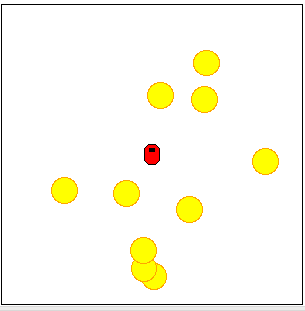
\includegraphics[scale=0.5]{environment.png}
\end{center}
\caption{In this experiment there are initially 10 light sources,
  representing food, which are randomly positioned within the
  environment.  The robot's goal is to stay alive for as long as
  possible by going to and consuming the light sources which provide
  energy.}
\label{environment}
\end{figure}

It is often useful to include figures here to show aspects of your
experiment.  For example, if you are using a simulation, include a
picture of the environment and the robot as in Figure~\ref{environment}.

In some cases, it may also be useful to include pseudocode (as shown
below) to explain how a particular variation of an algorithm that you
are exploring operates.

\begin{verbatim}
initialize the population with randomly weighted simple networks
for each generation
   speciate the population
   perform crossover within species
\end{verbatim}

\section{Results}

In this section you should illustrate the most interesting aspects of
the results using figures and tables.  For example, as see in
Figure~\ref{fitness}, the best performing network was discovered in
generation 22 by NEAT. Be sure that each figure and table includes a
caption.  Also be sure to refer to each figure and table in the main
text of the paper.

\begin{figure}[h]
\begin{center}
\fbox{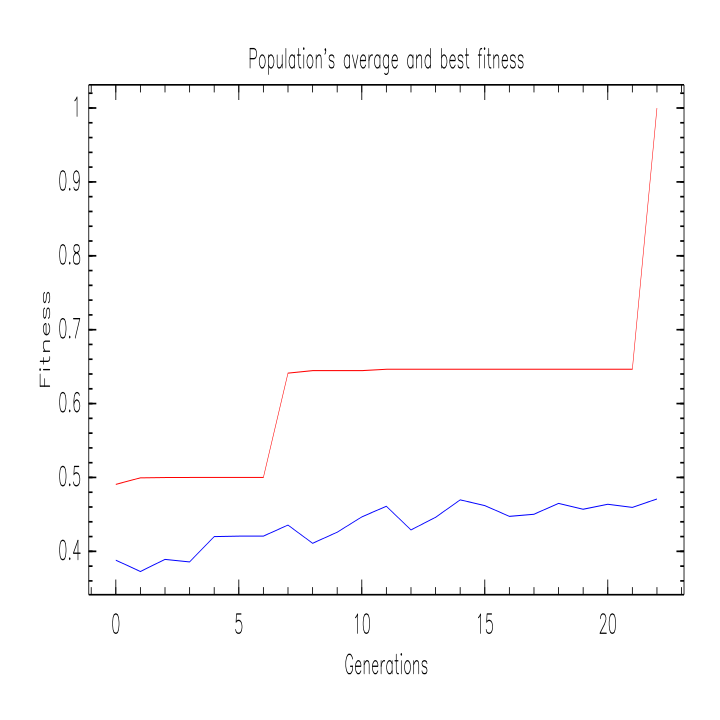
\includegraphics[scale=0.5]{avg_fitness.png}}
\fbox{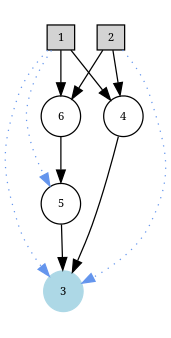
\includegraphics[scale=1]{phenotype.png}}
\end{center}
\caption{On the left: The average fitness (shown in blue) and the best
  fitness (shown in red) during one run of NEAT. On the right: The
  topology of the best network found.}
\label{fitness}
\end{figure}

\section{Discussion}

In this section you should discuss the significance of the results.
You should look at the bigger picture and place your experiment in the
context of the field as a whole.  

\bibliography{paper}
\bibliographystyle{plain}

\end{document}